% !TeX root = ../main.tex
\section{Capteur RTD Pt100 (PCA 1.1505.1M)}

\subsection{Mesure de résistance et étalonnage à \qty{0}{\degreeCelsius}}
% Mesures manuelles 2W vs 4W, étalonnage au bain sec Fluke et comparaison

\subsection{Temps de réponse du capteur dans l'eau}
\label{subsec:temps_reponse_pt100}

Afin de mesurer la dynamique de réponse du capteur Pt100 chemisé en inox, celui-ci a été brusquement plongé depuis la température ambiante dans un récipient d'eau chaude. L'acquisition a été effectuée en mode quatre fils (4W) via LabVIEW.

Les deux premiers points acquis avant le début effectif de l'immersion ont été retirés afin de synchroniser l'origine des temps ($t = \qty{0}{\second}$) avec le début réel du saut de température.

Le comportement dynamique est modélisé par un système linéaire du premier ordre :
\begin{equation}
    T(t) = T_\infty - (T_\infty - T_0) \cdot \exp\left(-\frac{t}{\tau}\right)
    \label{eq:premier_ordre}
\end{equation}
où $T_0 = \qty{24.11}{\degreeCelsius}$ est la température au déclenchement du saut, $T_\infty = \qty{66.71}{\degreeCelsius}$ la température finale asymptotique dans l'eau chaude, et $\tau$ la constante de temps recherchée.

\begin{figure}[H]
    \centering
    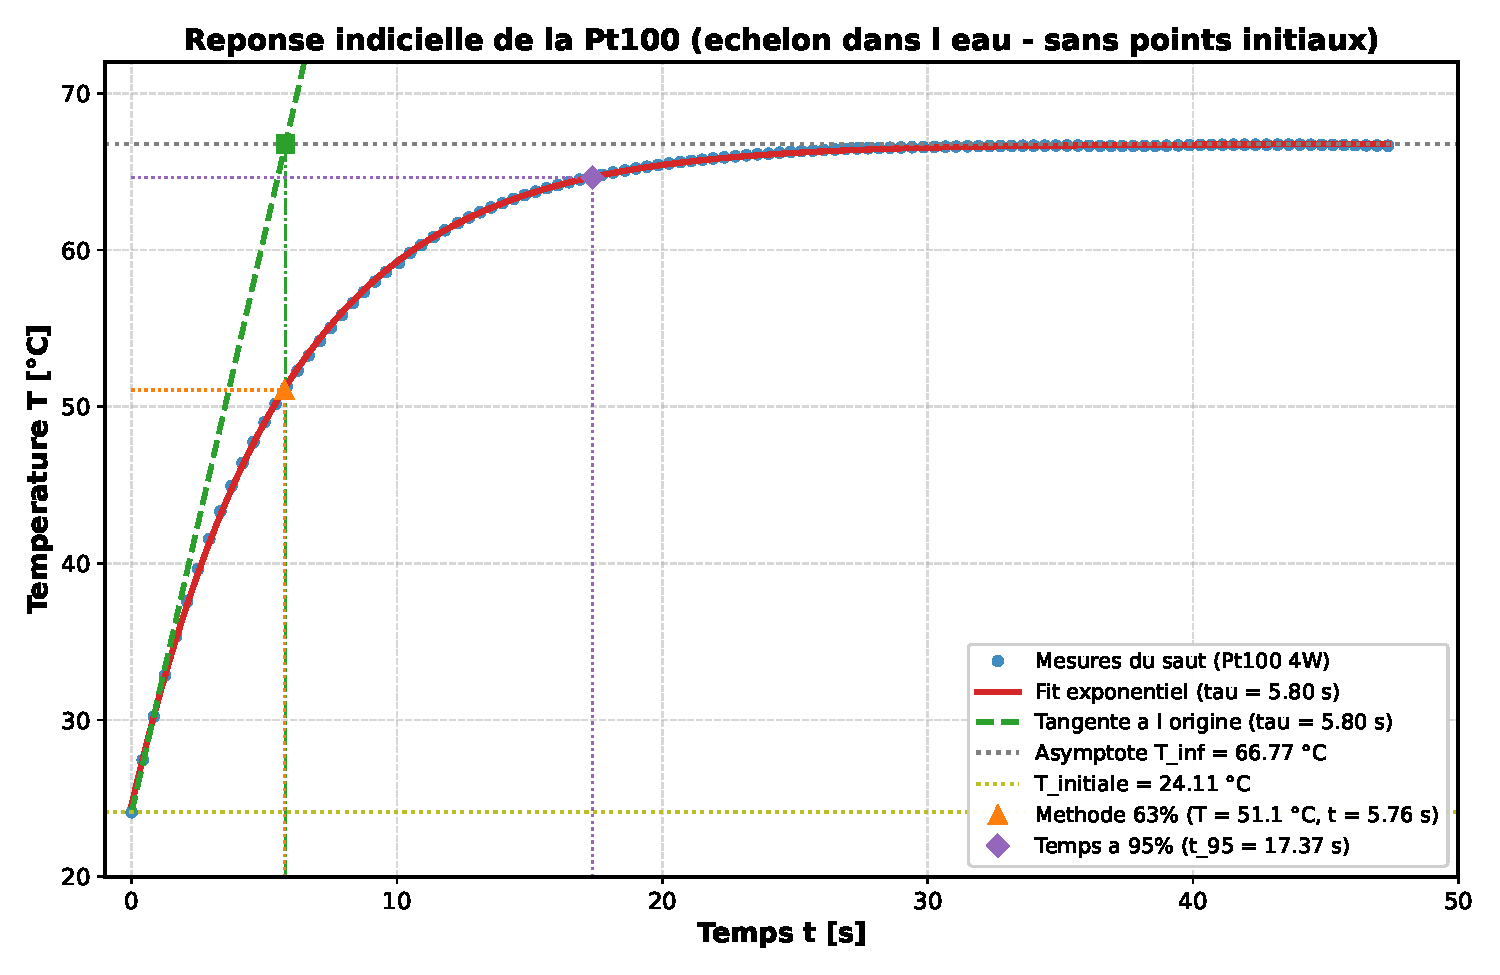
\includegraphics[width=0.92\textwidth]{assets/graphs/reponse_indicielle_pt100.pdf}
    \caption{Réponse indicielle de la sonde RTD Pt100 lors du saut de température dans l'eau chaude (sans les points initiaux hors eau) : comparaison des mesures, du fit exponentiel, de la tangente à l'origine et des seuils à 63\% et 95\%.}
    \label{fig:reponse_indicielle_pt100}
\end{figure}

\subsubsection*{Méthode 1 : Tangente au démarrage de la montée}
La tangente est tracée à l'origine du saut ($t = \qty{0}{\second}$). Sa pente initiale vaut :
\begin{equation}
    p = \left.\frac{\mathrm{d}T}{\mathrm{d}t}\right|_{t=0} = \frac{T_\infty - T_0}{\tau} \approx \qty{7.36}{\degreeCelsius\per\second}
\end{equation}
L'intersection de cette tangente avec l'asymptote horizontale $T = T_\infty$ donne directement la constante de temps :
\begin{equation}
    \tau_{\text{tan}} = \mathbf{\qty{5.80}{\second}}
\end{equation}

\subsubsection*{Méthode 2 : Seuil des 63\% de l'amplitude du saut}
Pour un système du premier ordre, la température atteint \qty{63.2}{\percent} de son saut total à $t = \tau$ :
\begin{equation}
    T_{63\%} = T_0 + 0.632 \cdot (T_\infty - T_0) = 24.11 + 0.632 \cdot (66.71 - 24.11) = \qty{51.07}{\degreeCelsius}
\end{equation}
Par interpolation sur les données de mesure, ce seuil est franchi à :
\begin{equation}
    \tau_{63\%} = \mathbf{\qty{5.76}{\second}}
\end{equation}

\subsubsection*{Méthode 3 : Fit exponentiel (moindres carrés)}
L'ajustement non-linéaire sur l'ensemble de la courbe du saut selon le modèle :
\begin{equation}
    T_{\text{fit}}(t) = A + B \cdot \exp\left(-\frac{t}{\tau_{\text{fit}}}\right)
\end{equation}
donne les paramètres optimaux :
\begin{itemize}[leftmargin=1.2cm]
    \item Asymptote : $A = T_\infty = \qty{66.77}{\degreeCelsius}$ ;
    \item Amplitude : $B = \qty{-42.19}{\degreeCelsius}$ ;
    \item Constante de temps optimale : $\mathbf{\tau_{\text{fit}} = \qty{5.80}{\second}}$ ;
    \item Écart quadratique moyen (RMSE) : $\text{RMSE} = \qty{0.09}{\degreeCelsius}$.
\end{itemize}

\subsubsection*{Méthode 4 : Temps de réponse à 95\%}
À partir de la constante de temps $\tau = \qty{5.80}{\second}$, le temps de réponse à \qty{95}{\percent} se calcule par :
\begin{equation}
    t_{95\%} = -\ln(0.05) \cdot \tau \approx 2.996 \cdot \tau \approx \mathbf{\qty{17.37}{\second}}
\end{equation}
Le capteur chemisé dans l'eau atteint ainsi \qty{95}{\percent} de sa température finale après \qty{17.37}{\second}.

\begin{table}[H]
    \centering
    \small
    \begin{tabularx}{0.85\textwidth}{Xcc}
        \toprule
        Méthode & Constante $\tau$ [s] & Écart relatif au fit [\%] \\
        \midrule
        Méthode 1 (Tangente à l'origine) & \qty{5.80}{\second} & \qty{0.0}{\percent} \\
        Méthode 2 (Seuil 63\%) & \qty{5.76}{\second} & \qty{-0.7}{\percent} \\
        Méthode 3 (Fit exponentiel) & \qty{5.80}{\second} & Référence \\
        \midrule
        Temps de réponse à 95\% ($t_{95\%}$) & \multicolumn{2}{c}{\textbf{\qty{17.37}{\second}}} \\
        \bottomrule
    \end{tabularx}
    \caption{Synthèse comparative des constantes de temps de la Pt100.}
    \label{tab:comparaison_tau}
\end{table}

\noindent
\textbf{Discussion :} Les résultats démontrent une excellente cohérence entre les méthodes (écart maximal inférieur à \qty{1}{\percent}). La constante de temps d'environ \qty{5.8}{\second} est propre aux échanges thermiques dans l'eau. Dans l'air, où le coefficient de convection est bien plus faible, le temps de réponse serait beaucoup plus long.
